\documentclass{beamer}
%\usepackage[latin1]{inputenc}
\usepackage[spanish]{babel}
\usepackage[T1]{fontenc}
\usepackage{style/slides}
\usepackage{graphicx,hyperref,url}
%\usefonttheme{serif}
%\setmainfont{Linux Libertine O}

\usepackage{subfiles}
\usepackage{subfigure}
\usepackage{pdfpages}
\usepackage{amsthm}
\usepackage{amsmath}
\usepackage{amssymb}

\usepackage{algorithm}
\usepackage{algorithmic}
\NeedsTeXFormat{LaTeX2e}
\ProvidesPackage{style/spanishAlgorithmic} [2017/04/25 Traducciones para el paquete de algoritmos]

\floatname{algorithm}{Algoritmo}
\renewcommand{\listalgorithmname}{\'Indice de algoritmos}
\renewcommand{\algorithmicrequire}{\textbf{Entrada:}}
\renewcommand{\algorithmicensure}{\textbf{Salida:}}
\renewcommand{\algorithmicend}{\textbf{fin}}
\renewcommand{\algorithmicif}{\textbf{si}}
\renewcommand{\algorithmicthen}{\textbf{entonces}}
\renewcommand{\algorithmicelse}{\textbf{si no}}
\renewcommand{\algorithmicelsif}{\algorithmicelse}
\renewcommand{\algorithmicendif}{\algorithmicend\ \algorithmicif}
\renewcommand{\algorithmicfor}{\textbf{para}}
\renewcommand{\algorithmicforall}{\textbf{para todo}}
\renewcommand{\algorithmicdo}{\textbf{hacer}}
\renewcommand{\algorithmicendfor}{\algorithmicend\ \algorithmicfor}
\renewcommand{\algorithmicwhile}{\textbf{mientras}}
\renewcommand{\algorithmicendwhile}{\algorithmicend\ \algorithmicwhile}
\renewcommand{\algorithmicloop}{\textbf{repetir}}
\renewcommand{\algorithmicendloop}{\algorithmicend\ \algorithmicloop}
\renewcommand{\algorithmicrepeat}{\textbf{repetir}}
\renewcommand{\algorithmicuntil}{\textbf{hasta que}}
\renewcommand{\algorithmicprint}{\textbf{imprimir}}
\renewcommand{\algorithmicreturn}{\textbf{devolver}}
\renewcommand{\algorithmictrue}{\textbf{cierto }}
\renewcommand{\algorithmicfalse}{\textbf{falso }}


\usepackage{tikz}
%\RequirePackage{tikz-uml}
%\RequirePackage{pgf-umlcd}
\usetikzlibrary{positioning,decorations.pathreplacing,shapes}
\usetikzlibrary{positioning,fit,babel,shapes.multipart,calc}
\usetikzlibrary{arrows.meta,bending}
\usetikzlibrary{external}

\theoremstyle{plain} % default
  \newtheorem{thm}{Teorema}
\theoremstyle{definition}
  \newtheorem{defn}{Definición}
  \newtheorem{exmp}{Ejemplo}

\def\unmedio{\frac{1}{2}}
\def\tonee{t_{(1)}}
\def\ttwo{t_{(2)}}
\def\tthree{t_{(3)}}
\def\RR{\mathbb{R}}
\def\ZZ{\mathbb{Z}}
\def\NN{\mathbb{N}}
\def\FF{\mathcal{F}}
\def\unitinterval{[0,1]}
\def\xinunitinterval{\forall x\in\unitinterval}
\def\xyinunitinterval{\forall x, y\in\unitinterval}
\def\tsucesion{t_i, t_j, \dots, t_l}
\def\tilda1{\tilde{1}}
\newcommand{\abs}[1]{\left\vert#1\right\vert}
\newcommand{\unitspace}{\unitinterval \rightarrow \unitinterval}

\newcommand{\REV}[1]{{\color{red}\Large#1}}
\newcommand{\MATLAB}{\textsc{MatLab}}
\newcommand{\bb}{\bfseries}

%\addbibresource{bibliografia.bib}

% The title of the presentation:
%  - first a short version which is visible at the bottom of each slide;
%  - second the full title shown on the title slide;
\title[Segmentación de imágenes con lógica difusa]{
  Segmentación de imágenes a través de lógica difusa y funciones REF, de Dombi y penalti}

% Optional: a subtitle to be dispalyed on the title slide
%\subtitle{Trabajo Fin de Grado}

% The author(s) of the presentation:
%  - again first a short version to be displayed at the bottom;
%  - next the full list of authors, which may include contact information;
\author[Iñigo Aguas Ardaiz]{
  I\~nigo Aguas Ardaiz \\\medskip\\[5mm]
  {\footnotesize Humberto Bustince Sola \\ Fco. Javier Fernández Fernández}}

% The institute:
%  - to start the name of the university as displayed on the top of each slide
%    this can be adjusted such that you can also create a Dutch version
%  - next the institute information as displayed on the title slide
\institute[Universidad P\'ublica de Navarra]{
Trabajo Fin de Grado\\
Grado en Ingeniería Informática\\
E.T.S. de Ing. Industrial, Informática y de Telecomunicación\\
Universidad Pública de Navarra}

% Add a date and possibly the name of the event to the slides
%  - again first a short version to be shown at the bottom of each slide
%  - second the full date and event name for the title slide
\date[25 de junio de 2015]{
25 de junio de 2015}

\begin{document}

\begin{frame}
  \titlepage
\end{frame}

\begin{frame}
  \frametitle{Outline}
  \tableofcontents
\end{frame}

% Section titles are shown in at the top of the slides with the current section
% highlighted. Note that the number of sections determines the size of the top
% bar, and hence the university name and logo. If you do not add any sections
% they will not be visible.
\section{Introducción}
\begin{frame}
  \bfseries\Large\centering  Introducción
\end{frame}

\begin{frame}
  \frametitle{Motivación}
  \begin{center}\Large
    ``?`Cómo podríamos siquiera {\em empezar} a explicar la substancia de tales problemas a una entidad que no sea ella misma consciente\dots?''
  \end{center}
  \begin{flushright}
    {\scshape R. Penrose}\\
    {\em La nueva mente del emperador}
  \end{flushright}
\end{frame}

\begin{frame}
  \frametitle{Definición del problema}
  \begin{figure}
    \centering
    \includegraphics[width=0.625\textwidth]{img/molino.jpg}
    \caption{Distinguir el molino del pueblo del fondo no es difícil para un humano aunque sí para una máquina.}
    \label{img:ejemplomolino}
  \end{figure}
\end{frame}

\begin{frame}
  \frametitle{Definición del problema}
  \begin{defn}\label{def:definicionproblema}
    Dada una imagen $Q$ que se puede subdividir en $n$ regiones $R_{1}, \dots, R_{n}$, y conocida $P$ que es una cierta propiedad booleana que cumplen todos los píxeles de la región $R_{i}, \forall  i=1,\dots ,n$, se deberá cumplir siempre que:
    \begin{enumerate}
      \item $\bigcup_{i=1}^{n}R_{i}=Q$;
      \item En una región $R_{i}, \forall i=1,\dots ,n$ todos sus píxeles están conectados;
      \item $R_{i}\cap R_{j}=\emptyset, \forall i, j : i\neq j;$
      \item $P(R_{i}) = \text{ VERDADERO }, \forall  i=1,\dots ,n;$
      \item $P(R_{i}\cup R_{j}) = \text{ FALSO }, \forall  i=1,\dots ,n.$
    \end{enumerate}
  \end{defn}
\end{frame}

\begin{frame}
  \frametitle{Ejemplos}
  \begin{figure}
    \centering
    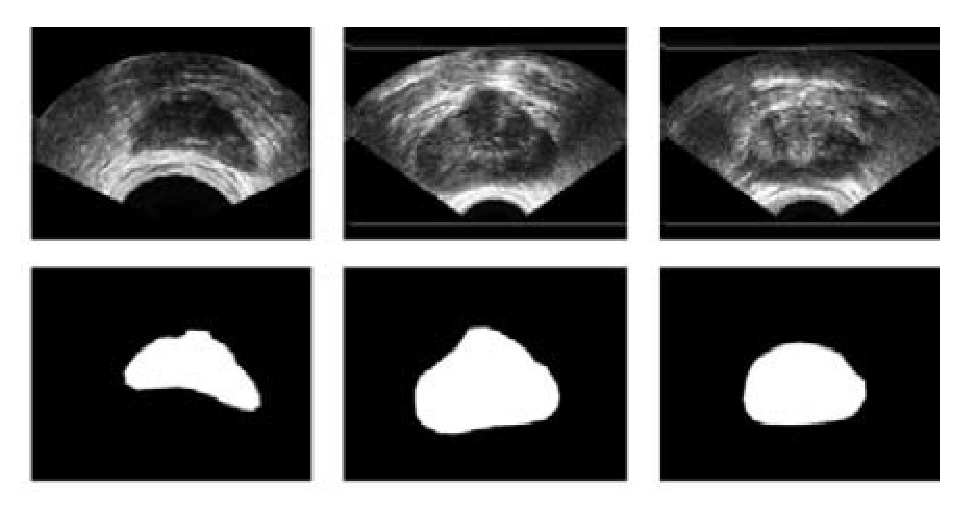
\includegraphics[width=0.7\textwidth]{img/imagenmedica.eps}
    \caption{Segmentación de una imagen de próstata.}
    \label{img:segmentacionmedica}
  \end{figure}
\end{frame}

\begin{frame}
  \frametitle{Ejemplos}
  \begin{figure}
  \centering
    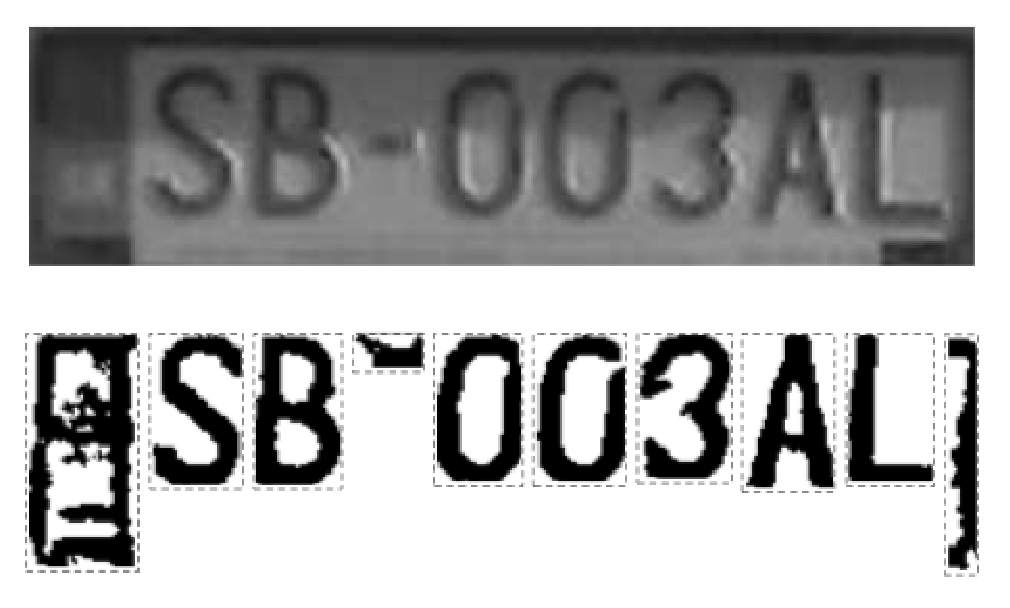
\includegraphics[width=0.5\textwidth]{img/matricula.eps}
    \caption{Utilización de técnicas de segmentación para extraer la información de una matrícula y poder ser procesada por un sistema de IA.}
    \label{img:matricula}
  \end{figure}
\end{frame}

\begin{frame}
  \frametitle{Objetivos}
  \begin{enumerate}
    \item Investigar y conocer técnicas actuales de segmentación de imagen.
    \item Implementar diferentes algoritmos de segmentación evaluando su mejora y tratando de generalizarlos.
    \begin{enumerate}
      \item Analizar y evaluar las funciones de J. Dombi. Sustituir por funciones REF construcción de los conjuntos difusos para conocer sus efectos.
      \item Umbralizar a través de la agregación de resultados y obtención del mejor con funciones penalti.
      \item Implementar algoritmos que incluyan la agregación OWA de la función original (media aritmética).
    \end{enumerate}
    \item Analizar todos los puntos anteriores a fin de concluir los resultados del trabajo así como dirimir si se ha podido conseguir cumplir el propósito inicial.
  \end{enumerate}
\end{frame}

\begin{frame}
  \frametitle{Fuentes}
  \begin{center}
  {\bfseries ``Image thresholding using restricted equivalence functions and maximizing the measures of similarity''}\\[5mm]
  H. Bustince, E. Barreneche y M. Pagola\\
  Fuzzy Sets and Systems 158 (2007) pág. 496-516
  \end{center}
\end{frame}


\section{Conceptos básicos}
\begin{frame}
  \bfseries\Large\centering  Conceptos básicos
\end{frame}

\begin{frame}
  \frametitle{Imágenes digitales}
  \begin{figure}
  \centering
    \subfigure[Niveles de gris]
    {\includegraphics[height=0.1\textwidth]{img/matriznivelesgris.jpg}}\quad
    \subfigure[Normalizada]
    {\includegraphics[height=0.1\textwidth]{img/matriznormalizada.jpg}}\quad\
    \subfigure[Gráfica]
    {\includegraphics[width=0.1\textwidth]{img/imagendigital.jpg}}
    \caption{Imagen digital en diferentes representaciones.}
    \label{fig:defimagen}
  \end{figure}

  \begin{defn}[Definición]
    Se define el histograma de una imagen $Q$ con niveles de gris en el intervalo [0, 255] como la función $h(q) = n_q$ donde $n_q$ es el número de píxeles en la imagen con la intensidad $q$.
  \end{defn}
\end{frame}

\begin{frame}
  \frametitle{Contraste}
  \begin{figure}
  \centering
      \subfigure[Imagen original]
      {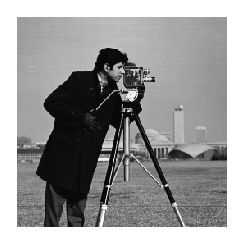
\includegraphics[width=0.3\textwidth]{img/camera.eps}}\quad
      \subfigure[Imagen con poco contraste]
      {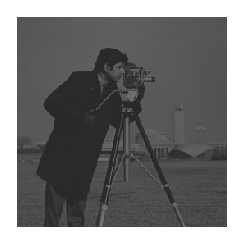
\includegraphics[width=0.3\textwidth]{img/camerabcon.eps}}\quad
      \subfigure[Imagen con muy poco contraste]
      {
\includegraphics[width=0.3\textwidth]{img/cameramuybcon.eps}}
      \caption{Imagen del fotógrafo con diferentes contrastes\label{fig:contraste}}
  \end{figure}
\end{frame}

\begin{frame}
  \frametitle{Ruido}
  \begin{figure}
  \centering
      \subfigure[Imagen original]
      {\includegraphics[width=0.3\textwidth]{img/lena}}\quad
      \subfigure[Imagen con ruido `sal y \mbox{pimienta}']
      {\includegraphics[width=0.3\textwidth]{img/lenas&p}}\quad
      \subfigure[Imagen con ruido gausiano]
      {\includegraphics[width=0.3\textwidth]{img/lenaga}}
      \caption{Imagen de Lena con diferentes tipo de ruido}
      \label{fig:defruido}
  \end{figure}
\end{frame}

%\begin{frame}   Hablar un poco pero sin decir mostrar nada.
%  \frametitle{Lógica clásica vs lógica difusa}
%\REV{¿Lógica difusa?}
%\end{frame}

\begin{frame}
  \frametitle{Funciones de Equivalencia Restringida (REF)}
  \begin{defn}\label{def:ref}
  Una función $REF  : [0, 1] \rightarrow [0, 1]$ es llamada de equivalencia restringida cuando cumple que:
    \begin{enumerate}
    \item $REF(x, y) = REF(y, x), \forall x, y \in [0, 1];$
    \item $REF(x, y) = 1$, si y sólo si, $x=y$;
    \item $REF(x, y) = 0$, si y sólo si, $x=1$ e $y=0$ ó si $x=0$ e $y=1$;
    \item $REF(x, y) = REF(c(x), c(y)),  \forall x, y \in [0, 1]$, siendo $c$ una negación fuerte.
    \item $\forall x, y, z \in [0, 1]$, si $x\leq y\leq z$, entonces $REF(x, y)\geq REF(x, z)$ y  $REF(y, z)\leq REF(x, z)$
    \end{enumerate}
  \end{defn}
\end{frame}

\begin{frame}{Funciones de Equivalencia Restringida (REF)}
  \begin{defn}\label{prop:contruccionref}
  Sean dos automorfismos $\varphi_{1}$ y $\varphi_{2}$, se llamará función $REF$ a la construcción que cumpla que:
  $$REF(x,y) = \varphi_1^{-1}(1-|\varphi_2(x)-\varphi_2(y)|) \quad\text{con}\quad c(x) = \varphi_2^{-1}(1-\varphi_2(x)).$$
  Además, si tenemos una $REF$ y un automorfismo en $\unitinterval$, la aplicación de estos ($F=\varphi \circ REF$) es otra $REF$.
  \end{defn}
\end{frame}

\begin{frame}{Funciones de agregación}
  %\frametitle{Funciones de agregación}
  \begin{defn}\label{def:agregacion}
  Se dice que $M : \unitinterval^n \rightarrow \unitinterval$ es una función de agregación de dimensión $n$ siempre que satisfaga:
    \begin{enumerate}
    \item $M(x_1, \dots, x_n) = 0$ si y sólo si $x_1=\dots=x_n=0$;
    \item $M(x_1, \dots, x_n) = 1$ si y sólo si $x_1=\dots=x_n=1$;
    \item $M$ es una función estrictamente creciente.
    \end{enumerate}
  \end{defn}
  \begin{defn}
  Una función de agregación $M$ será llamada media si
  $$ min(x_{1}, \dots, x_{n})  \leq M(x_{1}, \dots, x_{n}) \leq max(x_{1}, \dots, x_{n}).$$
  \end{defn}
\end{frame}

\begin{frame}
  \frametitle{Funciones OWA}
  \begin{defn}\label{def:owa}
  Una  función $F:\unitinterval^n\rightarrow\unitinterval$ será una función OWA de dimensión $n$ si existe un vector $w=(w_{1},w_{2},\dots,w_{n})\in \unitinterval^{n}$ tal que $\sum_{i}w_{i}=1$ de forma que
  $$F(x_{1},\dots,x_{n})=\sum^{n}_{j=1}w_{j}x_{\sigma(j)}$$
  donde $x_{\sigma(j)}$ es el $j$-ésimo mayor elemento del vector $(x_{1},\dots,x_{n})$.
  \end{defn}
\end{frame}
\begin{frame}{Funciones de agregación}
  \begin{equation*}\label{eq:pesosowamayoria}
   w_i = Q\left(\frac{i}{t+1}\right) - Q\left(\frac{i+1}{t+1}\right), \forall i\in \{1, \dots, n\}, \text{   sabiendo que}
  \end{equation*}
   $$Q(r) = \left\{\begin{aligned}
    0           &\quad \text{si}\quad r<0,5\\
    \frac{r-0,5}{0,5} &\quad \text{si}\quad 0,5\leq r\leq 1\\
    1           &\quad \text{si}\quad r>1\\
  \end{aligned}\right.$$
\end{frame}

\begin{frame}[squeeze]
  \frametitle{Funciones de similitud}
  \begin{defn}\label{def:similitud}
  Dada una función $M$ de agregación (definición \ref{def:agregacion}) y una función $REF$ (definición \ref{def:ref}) llamaremos a $SM$ función de similitud si $SM : \FF(X) \times \FF(X) \rightarrow [0,1]$ está definida tal que
  $$SM(A,B)=M^n_{i=1}REF(\mu_A(x_i), \mu_B(x_i))$$
  y satisface las siguientes condiciones:
    \begin{enumerate}
    \item $SM(A, B) = SM(B, A), \forall A, B \in \FF(X)$;
    \item $SM(A, A_c) = 0$, si y sólo si A no es difuso;
    \item $SM(A, B) = 1$ si y sólo si A = B;
    \item Si $A\leq B\leq C$, entonces $SM(A, B)\geq SM(A,C)$ y $SM(C, B)\geq SM(C,A)$;
    \item $SM(A_c, B_c) = SM(A,B)$
    \end{enumerate}
  \end{defn}
\end{frame}

\begin{frame}{Funciones penalty}
  \begin{defn}\label{def:penalti}
  La función $P:[a,b]^{n+1}\rightarrow \RR^{+} = [0, \infty]$ es una función penalti si y sólo si satiface que:
  \begin{enumerate}
    \item $P(x, y) \geq 0, \forall x, y$
    \item $P(x, y) = 0$ si $x_{i}=y \forall i=1,\dots ,n$
    \item $P(x,y)$ es cuasiconvexa en $y$ para cualquier $x$, esto es, $P(x, \lambda\cdot y_{1} +(1-\lambda)\cdot y_{2})\leq max(P(x, y_{1}), P(x, y_{2}))$.
  \end{enumerate}
  \end{defn}
\end{frame}

\begin{frame}{Funciones penalty}
  La función en la que se basan las penalti es $$f(x)=\arg min_{y} P(x,y)$$ si $y$ es el único mínimo e $y=\frac{a+b}{2}$ si el conjunto de minimizadores es el intervalo $(a, b)$.

  \begin{thm}
  Todas las funciones de agregación llamadas medias pueden ser escritas como una función basada en una función penalti expresada en la definición anterior.
  \end{thm}
\end{frame}

\begin{frame}[squeeze]{Funciones de Dombi}
  \begin{defn}\label{def:dombi}
  Dados $x=(x_1, x_2, \dots,x_n)$ y $w=(w_1,w_2,\dots,w_n)$, denotaremos $D$ como una función de equivalencia de Dombi cuando tengamos que
  $$D(w,x)=\frac{1}{2}\left(1+\prod(1-2x_{i})^{w_{i}}\right)$$
  \end{defn}
  \begin{block}{}\label{def:propiedadesdombi}
  La función de equivalencia de Dombi, $D$, cumple las siguientes propiedades:
  \begin{enumerate}
    \item $D:\unitinterval\times\unitspace \text{ es continua}$;
    \item $D((w_1,w_2),(0,0)) = 1$;\quad$D((w_1,w_2),(1,1)) = 1$;
    \item $D((w_1,w_2),(0,1)) = 0$;\quad$D((w_1,w_2),(1,0)) = 0$;
    \item $D((w_1,w_2),(x,c(x))) = 0$.
  \end{enumerate}
  \end{block}
\end{frame}

\begin{frame}{Algoritmo 1. Maximización de la similitud}
  \begin{algorithm}[H]%
  \begin{algorithmic}[1]
  \REQUIRE Una imagen $Q$ en escala de grises donde sus píxeles estén entre $0$ y $L-1$.
  \ENSURE El umbral $t$ a partir del cual se divide $Q$ en objeto y fondo.
  \FOR {$t$:=0 hasta $L-1$}
  \STATE Divisón de la imagen en dos clases $C_b(t)$ y $C_o(t)$. Para cada una de estas clases, calcular su media: $m_b(t)$ y $m_o(t)$.
  \STATE Construcción del conjunto difuso $Q_t$.
  \STATE Calcular la $SM(\tilda1, Q_t)$. \label{lin:alg1:similitud}
  \ENDFOR
  \RETURN \{$t$ | max($SM$)\}
  \end{algorithmic}
  \caption{Maximización de la similitud}\label{alg:algoritmo1}
  \end{algorithm}
\end{frame}

\begin{frame}{Algoritmo 1. Maximización de la similitud}
  \begin{defn}\label{def:mediasmonoumbral}
Teniendo en cuenta la definición de la media de una imagen que se ha dado, y disponiendo del histograma de la imagen $h(q)$ para un cierto nivel $q, \forall q\in Q$, se define la media de los píxeles del fondo como:
$$m_b(t)=\frac{\sum_{q=0}^{t}qh(q)}{\sum_{q=0}^{t}h(q)};$$
y para los píxeles del objeto como:
$$m_o(t)=\frac{\sum_{q=t+1}^{L-1}qh(q)}{\sum_{q=t+1}^{L-1}h(q)}.$$
\end{defn}
\end{frame}

\begin{frame}{Algoritmo 1. Maximización de la similitud}
\begin{defn}\label{def:conjuntodifusomonoumbral}
Dada $Q$, una imagen en la escala de L niveles de gris, y $t$, un nivel de gris de forma que $0\leq t\leq L-1$. Teniendo en cuenta que $F$ es una función $REF$ ya que la $REF \circ \varphi$ lo es, se define el conjunto
$$Q_t = \{(q, \mu_{Q_t}(q)|q\in \{0,1,\dots, L-1\}\}$$
teniendo en cuenta que
$$\mu_{Q_t}(q) = \left\{ \begin{aligned}
     \varphi\left(REF\left(\frac{q}{L-1}, \frac{m_b(t)}{L-1} \right)\right) & \quad\text{si}\ q\leq t,\\
     \varphi\left(REF\left(\frac{q}{L-1}, \frac{m_o(t)}{L-1} \right)\right) & \quad\text{si}\ q> t.
 \end{aligned}\right.$$
 \end{defn}
\end{frame}

\begin{frame}{Algoritmo 1. Maximización de la similitud}
  \begin{equation*} \label{eq:conjdifusosdombimono}
    \mu_{Q_t}(q) = \left\{ \begin{aligned}
         \frac{1}{2}\left(1 + \left(1-2\frac{q}{L-1}\right)^w\cdot\left(1-2\frac{m_b(t)}{L-1}\right)^w\right)& \quad\text{si}\ q\leq t,\\
         \frac{1}{2}\left(1 + \left(1-2\frac{q}{L-1}\right)^w\cdot\left(1-2\frac{m_o(t)}{L-1}\right)^w\right)& \quad\text{si}\ q> t.
     \end{aligned}\right.
\end{equation*}
\end{frame}

\begin{frame}[squeeze]
  \begin{algorithm}[H]%
  \begin{algorithmic}[1]
  \REQUIRE Una imagen $Q$ en escala de grises donde sus píxeles estén entre $0$ y $L-1$.
  \ENSURE El umbral $t$ a partir del cual se divide $Q$ en objeto y fondo.
  \FOR {$t$:=0 hasta $L-1$}
  \STATE \begin{equation*}\begin{split}
  A(Q_t)= \sum_{q=0}^{t} h(q)\varphi_1^{-1}\left(1-\abs{\varphi_2\left(\frac{q}{L-1}\right)-\varphi_2\left(\frac{m_b(t)}{L-1}\right)}\right) + \\ \sum_{q=t+1}^{L-1} h(q)\varphi_1^{-1}\left(1-\abs{\varphi_2\left(\frac{q}{L-1}\right)-\varphi_2\left(\frac{m_o(t)}{L-1}\right)}\right)
  \end{split}\end{equation*}
  \ENDFOR
  \RETURN \{$t$ | max($A(Q_t)$)\}
  \end{algorithmic}
  \caption{Umbralización del área}\label{alg:algoritmo2}
  \end{algorithm}
\end{frame}

\begin{frame}{Algoritmo 3. Selección del umbral óptimo.}
  \begin{algorithm}[H]%
  \begin{algorithmic}[1]
  \REQUIRE Una imagen $Q$ en escala de grises donde sus píxeles estén entre $0$ y $L-1$.
  \ENSURE El umbral óptimo $t^*$ a partir del cual se divide $Q$ en objeto y fondo.
  \FOR {$t$:=0 hasta $L-1$}
  \STATE Calcular los conjuntos $Q_t$ como se describe en la definición \ref{def:conjuntodifusomonoumbral}.
  \STATE Calcular los conjuntos $H$ como se muestra en la definición \ref{def:conjuntoHmonoumbral}.
  \STATE Calcular la $SM(Q_t, H(Q_t))$.
  \ENDFOR
  \RETURN \{$t*$ | max($SM$)\}
  \end{algorithmic}
  \caption{Selección del umbral óptimo}\label{alg:algoritmo3}
  \end{algorithm}
\end{frame}

\begin{frame}{Algoritmo 3. Selección del umbral óptimo.}
  \begin{defn}\label{def:conjuntoHmonoumbral}
  Dada $Q$, una imagen en la escala de L niveles de gris, y $t$, un nivel de gris de forma que $0\leq t\leq L-1$, se calcula su conjunto $H(Q_t)$ como
  $$H(Q_t) = \{(q, \mu_{H(Q_t)}(q)|q\in \{0,1,\dots, L-1\}\}$$
  teniendo en cuenta que
  $$\mu_{Q_t}(q) = \left\{ \begin{aligned}
      \frac{m_b(t)}{L-1} & \quad\text{si}\ q\leq t,\\
      \frac{m_o(t)}{L-1} & \quad\text{si}\ q> t.
   \end{aligned}\right.$$
   \end{defn}
\end{frame}

\begin{frame}{Otros métodos de segmentación}
  \begin{itemize}
    \item Umbralización global.
    \item Método de Otsu.
    \item Maximización de la entropía de Renyi.
    \item Clasificación {\em K-means}.
  \end{itemize}
\end{frame}

\section{Experimentos con funciones de Dombi}
\begin{frame}
  \bfseries\Large\centering  Experimentos con funciones de Dombi
\end{frame}

\begin{frame}{Experimentos con funciones de Dombi}
  \begin{block}{Explicación del experimento}
    Sustitución de las funciones REF en la construcción de los conjuntos difusos con funciones de Dombi.
  \end{block}
  \begin{itemize}
    \item Experimentos con casi 30 imágenes.
    \item Diferentes histogramas, ruidos y contrastes.
  \end{itemize}
  \begin{block}{Error cuadrático medio}
    $$ECM(Q, Q') = \frac{\sum_{x=1}^N\sum_{y=1}^M \left(q(x,y)-q'(x,y)\right)^2}{N\cdot M}.$$
  \end{block}
\end{frame}

\begin{frame}[squeeze]{Experimentación}
  \begin{table}
  \centering
    \begin{tabular}{ccccc}\hline
    \includegraphics[width=0.15\textwidth]{img/orig/chair.jpg} &
    \includegraphics[width=0.15\textwidth]{img/orig/block.jpg} &
    \includegraphics[width=0.15\textwidth]{img/orig/02.jpg} &
    \includegraphics[width=0.15\textwidth]{img/orig/09.jpg} &
    \includegraphics[width=0.15\textwidth]{img/orig/07.jpg}\\
    \end{tabular}\\
    \begin{tabular}{ccc}
    \includegraphics[width=0.15\textwidth]{img/orig/chairga.jpg} &
    \includegraphics[width=0.15\textwidth]{img/orig/chairsp005.jpg} &
    \includegraphics[width=0.15\textwidth]{img/orig/chairsp020.jpg}\\
    \end{tabular}\\
    \begin{tabular}{cc}
    \includegraphics[width=0.15\textwidth]{img/orig/chairbcon.jpg} &
    \includegraphics[width=0.15\textwidth]{img/orig/chairmuybcon.jpg}\\\hline
    \end{tabular}
  \caption{Imágenes originales.}
  \end{table}
\end{frame}

\begin{frame}{Resultados al sustituir la función REF en el Algoritmo 1}
  \begin{table}
  \centering
  \begin{tabular}{c||c|c|c|c|c}
  $\mathbf{w}$    &\bb Silla&\bb Bloques&\bb Engranaje&\bb Letras&\bb Sombra\\\hline\hline
  $\mathbf{0,1}$  &   218   &    255    &     250     &   142    &   200  \\\hline
  $\mathbf{0,5}$  &   226   &    255    &     250     &    39    &   230  \\\hline
  $\mathbf{0,75}$ &    95   &    119    &     115     &   103    &   111  \\\hline
  $\mathbf{1}$    &   127   &    123    &     137     &   160    &   125  \\\hline
  $\mathbf{1,25}$ &    70   &     97    &      96     &    80    &    91  \\\hline
  $\mathbf{1,5}$  &    45   &     79    &      0      &    39    &    64  \\\hline
  $\mathbf{2}$    &   144   &     76    &     138     &   197    &    96  \\\hline
  $\mathbf{5}$    &   218   &     31    &      59     &   216    &   219  \\\hline
  \end{tabular}
  \caption{Umbrales de cada imagen con la función de Dombi y diferentes $w$.\label{tab:resultexp1dombi}}
  \end{table}
\end{frame}

\begin{frame}{Resultados al sustituir la función REF en el Algoritmo 1}
  \begin{table}
  \centering
  \begin{tabular}{c||c|c|c}
  $\mathbf{REF_1=1-\abs{x-y}}$ & $\mathbf{w=0,75}$ &\bb $\mathbf{w=1}$ &\bb $\mathbf{w=1,25}$\\\hline\hline
  \includegraphics[width=0.2\textwidth]{img/res/e1a/alg1tipo1-chair.jpg} &
  \includegraphics[width=0.2\textwidth]{img/res/e1a/alg1tipo6-chair.jpg} &
  \includegraphics[width=0.2\textwidth]{img/res/e1a/alg1tipo6d0.75-chair.jpg} &
  \includegraphics[width=0.2\textwidth]{img/res/e1a/alg1tipo6d1.25-chair.jpg} \\
  \includegraphics[width=0.2\textwidth]{img/res/e1a/alg1tipo1-09.jpg} &
  \includegraphics[width=0.2\textwidth]{img/res/e1a/alg1tipo6-09.jpg} &
  \includegraphics[width=0.2\textwidth]{img/res/e1a/alg1tipo6d0.75-09.jpg} &
  \includegraphics[width=0.2\textwidth]{img/res/e1a/alg1tipo6d1.25-09.jpg} \\\hline
  \end{tabular}
  \caption{Resultado de las segmentaciones para el algoritmo con REF y Dombi con varios $w = \{0,75; 1; 1,25\}$.\label{tab:resultexp1imagenesdombi}}
  \end{table}
\end{frame}

\begin{frame}{Resultados al sustituir la función REF en el Algoritmo 1}
  \begin{table}
  \centering
  \begin{tabular}{c||c|c|c}
             &\bb R. gausiano&\bb R. impulsivo 0.05&\bb R. impulsivo 0.2\\\hline\hline
  $\mathbf{0,1}$  &   219   &    226    &     226     \\\hline
  $\mathbf{0,5}$  &   234   &    226    &     242     \\\hline
  $\mathbf{0,75}$ &    99   &     95    &      95     \\\hline
  $\mathbf{1}$    &   128   &    127    &     127     \\\hline
  $\mathbf{1,25}$ &    74   &     70    &      62     \\\hline
  $\mathbf{1,5}$  &    35   &     45    &      37     \\\hline
  $\mathbf{2}$    &   147   &    136    &     127     \\\hline
  $\mathbf{5}$    &   226   &    218    &     226     \\\hline
  \end{tabular}
  \caption{Umbrales para las imágenes con ruido con la función de Dombi y diferentes valores de $w$.\label{tab:resultexp1ruido}}
  \end{table}
\end{frame}

\begin{frame}{Resultados al sustituir la función REF en el Algoritmo 1}
  \begin{table}
  \centering
  \begin{tabular}{c||c|c|c}
  $\mathbf{REF_1=1-\abs{x-y}}$ & $\mathbf{w=0,75}$ &\bb $\mathbf{w=1}$ &\bb $\mathbf{w=1,25}$\\\hline\hline
  \includegraphics[width=0.2\textwidth]{img/res/e1a/alg1tipo1-chairga.jpg} &
  \includegraphics[width=0.2\textwidth]{img/res/e1a/alg1tipo6-chairga.jpg} &
  \includegraphics[width=0.2\textwidth]{img/res/e1a/alg1tipo6d0.75-chairga.jpg} &
  \includegraphics[width=0.2\textwidth]{img/res/e1a/alg1tipo6d1.25-chairga.jpg} \\
  \includegraphics[width=0.2\textwidth]{img/res/e1a/alg1tipo1-chairsp005.jpg} &
  \includegraphics[width=0.2\textwidth]{img/res/e1a/alg1tipo6-chairsp005.jpg} &
  \includegraphics[width=0.2\textwidth]{img/res/e1a/alg1tipo6d0.75-chairsp005.jpg} &
  \includegraphics[width=0.2\textwidth]{img/res/e1a/alg1tipo6d1.25-chairsp005.jpg} \\\hline
  \end{tabular}
  \caption{Umbrales para las imágenes con ruido con otras versiones de algoritmos.\label{tab:resultexp1imagenesruido}}
\end{table}
\end{frame}

\begin{frame}{Algoritmo 1 con funciones penalti}
  \centering
  \includegraphics[width=10cm]{graficos/esquemaPenalti.pdf}
\end{frame}

\begin{frame}{Algoritmo 1 con funciones penalti}
  \begin{table}
  \centering
  \begin{tabular}{cc}\hline
  \includegraphics[width=0.2\textwidth]{img/res/e2a/alg1agregate-chair.jpg} &
  \includegraphics[width=0.2\textwidth]{img/res/e2a/alg1agregate-block.jpg} &
  \end{tabular}\\
  \begin{tabular}{ccc}
  \includegraphics[width=0.2\textwidth]{img/res/e2a/alg1agregate-02.jpg} &
  \includegraphics[width=0.2\textwidth]{img/res/e2a/alg1agregate-09.jpg} &
  \includegraphics[width=0.2\textwidth]{img/res/e2a/alg1agregate-07.jpg}\\\hline
  \end{tabular}
  \caption{Resultado para el nuevo algoritmo a través de penalti con todas las funciones propuestas.\label{tab:resultexp2imagenagregado}}
  \end{table}
\end{frame}

\begin{frame}{Algoritmo 3 con funciones de Dombi}
  \begin{table}
  \centering
  \begin{tabular}{c||c|c|c|c|c}
               &\bb Silla&\bb Bloques&\bb Engranaje&\bb Letras&\bb Sombra\\\hline\hline
  \bb Alg. 3A  &   115   &    80    &     88      &    199   &    121   \\\hline
  \bb Alg. 3B  &   127   &    123    &     84      &    200   &    125   \\\hline
  \bb Alg. 3C  &   218   &    254    &     250     &    142   &    219   \\\hline
  \end{tabular}
  \caption{Umbrales para cada imagen con el algoritmo 3 en todas sus nuevas versiones.\label{tab:resultexp3dombi}}
  \end{table}
\end{frame}

\begin{frame}{Reestructuración de los algoritmos}
  \begin{block}{Propiedades de funciones de equivalencia}
  Sea $e$ una función de equivalencia,
  \begin{enumerate}
    \item $e:\unitinterval\times\unitspace$ es continua;
    \item $e(0,0)=1$,\quad$e(1,1)=1$;
    \item $e(0,1)=0$,\quad$e(1,0)=0$;
    \item $e(x,x)=1$;
    \item $e(x,c(x))=0$.
  \end{enumerate}
  \end{block}
\end{frame}

\begin{frame}{Reestructuración de los algoritmos}
  \begin{exampleblock}{Solución}
  \begin{equation*}\label{eq:intentodesolucionardombi}
    \mu_{Q_t}(q)=\left\{ \begin{split}
                 min\left( 1, \frac
                    {\unmedio \left(1+\left(1-\frac{2q}{L-1}\right)\left(1-\frac{2m_b}{L-1}\right)\right)}
                    {\unmedio \left(1+\left(1-\frac{2m_b}{L-1}\right)\left(1-\frac{2m_b}{L-1}\right)\right)}\right)
                 \text{\quad si\quad} q\leq t\\
                 min\left( 1, \frac
                    {\unmedio \left(1+\left(1-\frac{2q}{L-1}\right)\left(1-\frac{2m_o}{L-1}\right)\right)}
                    {\unmedio \left(1+\left(1-\frac{2m_o}{L-1}\right)\left(1-\frac{2m_o}{L-1}\right)\right)}\right)
                \text{\quad si\quad} q > t
                \end{split}\right.
\end{equation*}
  \end{exampleblock}
\end{frame}

\section{Experimentos con funciones OWA}
\begin{frame}
  \bfseries\Large\centering  Experimentos con funciones OWA
\end{frame}

\begin{frame}
  \frametitle{Experimentos con funciones OWA}
    \begin{block}{Explicación del experimento}
    Sustitución de las medias por funciones OWA para la construcción de los conjuntos difusos.
  \end{block}
  \begin{itemize}
    \item {\bb Insertar datos normalizados}.
    \item Utilización del OWA `de la mayoría'.
  \end{itemize}
  \begin{block}{}
  {\bb Construcción del vector de pesos, $w$}\\
  Si tenemos un conjunto $C=\{c_1,\dots,c_6\}$, entonces el vector de pesos tendrá la forma $(0,0,0,\frac{1}{3},\frac{1}{3},\frac{1}{3})$.
  \end{block}
\end{frame}

\begin{frame}{Algoritmo 1. Maximización de la similitud}
  \begin{defn}\label{def:mediasmonoumbral}
Teniendo en cuenta la definición de la media de una imagen que se ha dado, y disponiendo del histograma de la imagen $h(q)$ para un cierto nivel $q, \forall q\in Q$, se define la media de los píxeles del fondo como:
$$m_b(t)=\frac{\sum_{q=0}^{t}qh(q)}{\sum_{q=0}^{t}h(q)};$$
y para los píxeles del objeto como:
$$m_o(t)=\frac{\sum_{q=t+1}^{L-1}qh(q)}{\sum_{q=t+1}^{L-1}h(q)}.$$
\end{defn}
\end{frame}

\begin{frame}[squeeze]{Algoritmo 1 con funciones OWA}
  \begin{table}
  \centering
  \resizebox*{0.90\textwidth}{!}{
  \begin{tabular}{c||c|c|c}
  \bfseries Silla                                &\bb Media&\bb OWA (1)&\bb OWA (2)\\\hline\hline
  \bb Alg. 1 con $\mathbf{REF_1=1-\abs{x-y}}$         &   127 &   50  &   50  \\\hline
  \bb Alg. 1 con $\mathbf{REF_1=1-\abs{x-y}^2}$       &   127 &   50  &   246 \\\hline
  \bb Alg. 1 con $\mathbf{REF_1=1-\abs{x-y}^{0.5}}$   &   119 &   50  &   50  \\\hline
  \bb Alg. 1 con $\mathbf{REF_1=(1-\abs{x-y})^2}$     &   127 &   50  &   50  \\\hline
  \bb Alg. 1 con $\mathbf{REF_1=(1-\abs{x-y})^{0.5}}$ &   127 &   50  &   50  \\\hline
  \multicolumn{4}{c}{}\\
  \bfseries Letras                               &\bb Media&\bb OWA (1)&\bb OWA (2)\\\hline\hline
  \bb Alg. 1 con $\mathbf{REF_1=1-\abs{x-y}}$         &   187 &   255 &   239 \\\hline
  \bb Alg. 1 con $\mathbf{REF_1=1-\abs{x-y}^2}$       &   174 &   255 &   239 \\\hline
  \bb Alg. 1 con $\mathbf{REF_1=1-\abs{x-y}^{0.5}}$   &   200 &   255 &   239 \\\hline
  \bb Alg. 1 con $\mathbf{REF_1=(1-\abs{x-y})^2}$     &   190 &   255 &   236 \\\hline
  \bb Alg. 1 con $\mathbf{REF_1=(1-\abs{x-y})^{0.5}}$ &   186 &   255 &   255 \\\hline
  \end{tabular}}
  \caption{Umbrales para todas las versiones del algoritmo 1 con la aplicación de OWA.\label{tab:resultexp4dombi}}
  \end{table}
\end{frame}

\begin{frame}{Algoritmo 2 con funciones OWA}
  \begin{table}
\centering\resizebox*{0.95\textwidth}{!}{
\begin{tabular}{c||c|c|c}
\bb Silla                                &\bb Media&\bb OWA (1)&\bb OWA (2)\\\hline\hline
\bb Alg. 2 con $\mathbf{\varphi_1=\varphi_2=x}$     &   119 &   50  &   50  \\\hline
\bb Alg. 2 con $\mathbf{\varphi_1=x^2 \text{ y }\varphi_2=x}$   &   119 &   58  &   50  \\\hline
\bb Alg. 2 con $\mathbf{\varphi_1=x^{0,5} \text{ y }\varphi_2=x}$     &   103 &   114 &   172 \\\hline
\bb Alg. 2 con $\mathbf{\varphi_1=1-\sqrt{1-x} \text{ y }\varphi_2=x}$  &   127 &   50  &   50  \\\hline
\multicolumn{4}{c}{}\\
\bb Letras                               &\bb Media&\bb OWA (1)&\bb OWA (2)\\\hline\hline
\bb Alg. 2 con $\mathbf{\varphi_1=\varphi_2=x}$     &   121 &   46  &   85  \\\hline
\bb Alg. 2 con $\mathbf{\varphi_1=x^2 \text{ y }\varphi_2=x}$   &   121 &   54  &   86  \\\hline
\bb Alg. 2 con $\mathbf{\varphi_1=x^{0,5} \text{ y }\varphi_2=x}$     &   101 &   136 &   136 \\\hline
\bb Alg. 2 con $\mathbf{\varphi_1=1-\sqrt{1-x} \text{ y }\varphi_2=x}$  &   123 &   255 &   231 \\\hline
\end{tabular}}
\caption{Umbrales para todas las versiones del algoritmo 2 con la aplicación de OWA.\label{tab:resultexp5dombi}}
\end{table}
\end{frame}

\begin{frame}{Algoritmo 1 con funciones penalti y OWA}
  \begin{table}
  \centering
  \begin{tabular}{c|c|c}
  \bb Media&\bb OWA (1)&\bb OWA (2)\\\hline\hline
  \includegraphics[width=0.15\textwidth]{img/res/e6/alg1agregadoowa1chair.jpg} &
  \includegraphics[width=0.15\textwidth]{img/res/e6/alg1agregadoowa2chair.jpg} &
  \includegraphics[width=0.15\textwidth]{img/res/e6/alg1agregadoowa3chair.jpg} \\\hline
  \includegraphics[width=0.15\textwidth]{img/res/e6/alg1agregadoowa1block.jpg} &
  \includegraphics[width=0.15\textwidth]{img/res/e6/alg1agregadoowa2block.jpg} &
  \includegraphics[width=0.15\textwidth]{img/res/e6/alg1agregadoowa3block.jpg} \\\hline
  \includegraphics[width=0.15\textwidth]{img/res/e6/alg1agregadoowa109.jpg} &
  \includegraphics[width=0.15\textwidth]{img/res/e6/alg1agregadoowa209.jpg} &
  \includegraphics[width=0.15\textwidth]{img/res/e6/alg1agregadoowa309.jpg} \\\hline
  \end{tabular}
  \caption{Resultados gráficos para la versión agregada del algoritmo 1 con la aplicación de OWA. \label{tab:resultexp6imagenes}}
  \end{table}
\end{frame}

\begin{frame}{Algoritmo 3 con funciones OWA}
  \begin{table}
  \centering
  \begin{tabular}{c||c|c|c}
Silla                                &\bb Media&\bb OWA (1)&\bb OWA (2)\\\hline\hline
\bb Alg. 3 (a)  &
\includegraphics[width=0.2\textwidth]{img/res/e7/alg3aowa1chair.jpg} &
\includegraphics[width=0.2\textwidth]{img/res/e7/alg3aowa2chair.jpg} &
\includegraphics[width=0.2\textwidth]{img/res/e7/alg3aowa3chair.jpg} \\
\bb Alg. 3 (b)  &
\includegraphics[width=0.2\textwidth]{img/res/e7/alg3bowa1chair.jpg} &
\includegraphics[width=0.2\textwidth]{img/res/e7/alg3bowa2chair.jpg} &
\includegraphics[width=0.2\textwidth]{img/res/e7/alg3bowa3chair.jpg} \\\hline
  \end{tabular}
  \caption{Resultados gráficos para la versión agregada del algoritmo 1 con la aplicación de OWA.}
  \end{table}
\end{frame}

\begin{frame}{Algoritmo 3 con funciones OWA}
  \begin{table}
  \centering
  \begin{tabular}{c||c|c|c}
Letras                               &\bb Media&\bb OWA (1)&\bb OWA (2)\\\hline\hline
\bb Alg. 3 (a)  &
\includegraphics[width=0.2\textwidth]{img/res/e7/alg3aowa109.jpg} &
\includegraphics[width=0.2\textwidth]{img/res/e7/alg3aowa209.jpg} &
\includegraphics[width=0.2\textwidth]{img/res/e7/alg3aowa309.jpg} \\
\bb Alg. 3 (b)  &
\includegraphics[width=0.2\textwidth]{img/res/e7/alg3bowa109.jpg} &
\includegraphics[width=0.2\textwidth]{img/res/e7/alg3bowa209.jpg} &
\includegraphics[width=0.2\textwidth]{img/res/e7/alg3bowa309.jpg} \\\hline
  \end{tabular}
  \caption{Resultados gráficos para la versión agregada del algoritmo 1 con la aplicación de OWA.}
  \end{table}
\end{frame}


\section{Conclusiones y líneas futuras}
\begin{frame}
  \bfseries\Large\centering  Conclusiones y líneas futuras
\end{frame}

\begin{frame}
  \frametitle{Conclusión y líneas futuras}
  \begin{itemize}\pause
    \item El ruido se mantiene. Utilización de filtros.\pause
    \item Mismo $w$ produce el mismo resultado para imágenes con y sin ruido y con diferencias de contrastes.\pause
    \item La función penlati consume el doble de tiempo.\pause
    \item Las funciones de Dombi no son adecuadas directamente para {\em fuzzificar} conjuntos. Pregunta abierta: ?`Existe un parámetro que entrenado podría dar buenas soluciones?\pause
    \item Las OWA para los conjuntos difusos que representan imágenes no son buenos.\pause
    \item La OWA sin frecuencia obtiene buenos resultados para la creación del conjunto H que se utiliza en el algoritmo 3 para el cálculo de la similitud.\pause
    \item Pregunta abierta: ?`Problemas en la creación de los OWA cuando se tiene que $h(q)=h(q')$?\pause
  \end{itemize}
\end{frame}

\begin{frame}
  \titlepage
\end{frame}

\end{document}
